 %!Author = Camilo Nuñez
%! Date = 9.06.2022

% Preamble
\documentclass[11pt]{article}

% Packages
\usepackage{amsmath}
\DeclareMathOperator*{\argmax}{argmax}

\usepackage{graphicx}
\graphicspath{ {../images/} }

%%%Mis paquetes
\usepackage{xcolor}
\def\red{\color{red}}
\usepackage{amsfonts}

%Title
\title{RL Excercises Chapter 4}

% Document
\begin{document}

    \maketitle
    \setcounter{section}{3}


    \section{Exercises}

    \subsection{Question}
    In Example 4.1, if Pİ is the equiprobable random policy, what is q pi (11, down)?
    What is q pi (7, down)?

    \subsection*{Answer}

    $ q_\pi(s,a) = \sum_{r \in \mathcal{R}; s' \in \mathcal{S}} r*p(s',r|s,a) + \gamma v_\pi (s') $

    where reward is always -1 and rewards are not discounted.

    $ q_\pi(s,a) = -1 + v_\pi (s') $

    $ q_\pi(11,down) = -1 + v_\pi (15) = -1 + 0 = -1  $

    $ q_\pi(7,down) = -1 + v_\pi (11) = -1 + (-14) = -15 $ ( $v_\pi (11)$  is looked up from figure 4.1 )

    \subsection{Question}

    In Example 4.1, suppose a new state 15 is added to the gridworld just below state 13, and its actions, left, up, right, and down, take the agent to states 12, 13, 14, and 15, respectively.
    Assume that the transitions from the original states are unchanged.
    What, then, is v pi (15) for the equiprobable random policy?
    Now suppose the dynamics of state 13 are also changed, such that action down from state 13 takes the agent to the new state 15.
    What is v pi (15) for the equiprobable random policy in this case?

    \subsection*{Answer}

    $ v_\pi(s) = \sum_{a \in \mathcal{A}} \pi(a|s) \sum_{r \in \mathcal{R}; s' \in \mathcal{S}} [p(s´,r|s,a) + \gamma v_\pi (s')] $

    where actions are equaprobable, reward is always -1 and rewards are not discounted.

    In first case, the new state is not reachable from state 13.

    $ v_\pi(s) = \sum_{a} 0.25 [(-1) + v_\pi (s')] $

    where $ v(12)=-22, v(13)=-20, v(14)=-14, v(9) = -20 $ :

    $ v_\pi(15) = (-1) + 0.25 * [v_\pi (12) + v_\pi (13) + v_\pi (14) + v_\pi (15) ] $

    $ v_\pi(15) = -15 + 0.25 v_\pi (15) = -20 $

    In second case, the new state is reachable from state 13.
    Now value of 13 depends on value of 15, and value of 15 depends on value of 13.
    We have two equations with two unknowns which can be solved.

    $v_\pi(15)$ is :

    $ v_\pi(15) = (-1) + 0.25 * [v_\pi (12) + v_\pi (13) + v_\pi (14) + v_\pi (15) ] $

    $ v_\pi(15) = -1 + 0.25 * [-36 + v_\pi (13) + v_\pi (15) ] = -1 -9 + \frac{v_\pi (13)}{4}  + \frac{v_\pi (15)}{4}$

    $ v_\pi(15) = \frac{ -40 + v_\pi (13) }{3}$

    $v_\pi(13)$ is :

    $ v_\pi(13) = (-1) + 0.25 * [v_\pi (12) + v_\pi (9) + v_\pi (14) + v_\pi (15) ] $

    $ v_\pi(13) = -1 + 0.25 * [-56 + v_\pi (15) ] = -1 -14 + \frac{v_\pi (15)}{4} =  -15 + \frac{v_\pi (15)}{4} $

    One can plug $ v_\pi(13) $ to obtain $ v_\pi(15) $ :

    $ v_\pi(15) = \frac{ -40 + -15 + \frac{v_\pi (15)}{4} }{3} = -20$

    \subsection{Question}

    What are the equations analogous to (4.3), (4.4), and (4.5) for the action-value function q pi and its successive approximation by a sequence of functions q 0 , q 1 , q 2 , . . .?

    \subsection*{Answer}

    \begin{equation}
        q_{\pi}(s, a) = E_\pi [R_{t+1} + \sum_{a'}  \gamma  \pi(a|S_{t+1}) q_{\pi} (S_{t+1}, a') | S_t = s, A_t = a]
    \end{equation}

    \begin{equation}
        q_{\pi}(s, a) = \sum_{s',r} p(s', r | s, a) [r + \sum_{a'} \gamma \pi(a|S_{t+1}) q_\pi(s', a')]
    \end{equation}

    \begin{equation}
        \label{eqn:eq4_5}
        q_{k+1}(s, a) = \sum_{s',r} p(s', r | s, a) [r + \sum_{a'} \gamma \pi(a|S_{t+1}) q_k(s', a')]
    \end{equation}

    \subsection{Question}

    The policy iteration algorithm on page 80 has a subtle bug in that it may never terminate if the policy continually switches between two or more policies that are equally good.
    This is ok for pedagogy, but not for actual use.
    Modify the pseudocode so that convergence is guaranteed.

    \subsection*{Answer}

    If $old-action \neq \pi(s)$, then policy-stable=false

    This expression may result in choosing between equally good actions causing the policy improvement step not to stop.

    Assuming the policy function assigns zero probabilities to all sub-optimal functions and return a set of optimal actions with uniform probability of being chosen. A possible solution could be:

    If $old-action \notin \pi(s)$, then policy-stable=false

    \subsection{Question}

    How would policy iteration be defined for action values?
    Give a complete algorithm for computing q * , analogous to that on page 80 for computing v * .
    Please pay special attention to this exercise, because the ideas involved will be used throughout the rest of the book.

    \subsection*{Answer}

    \subsubsection*{Policy Evaluation}
    Loop for each $ s \in S $: \\

    \hspace{4mm} Loop for each $ a \in A(s) $: \\

    \hspace{6mm} $q_{k+1}(s, a) = \mathbb{E}_{\pi}[R_{t+1}+\gamma v_k(S_{t+1})|S_t=s,A_t=a]$
    
    \hspace{6mm} $= \sum_{s',r} p(s',r| s, a) [ r + \gamma Q(s', \pi(s'))  ] $

    \subsubsection*{Policy Improvement}
    \hspace{4mm} $ \pi(s) = \argmax_{a} q(s, a) $

    \subsection{Question}

    Suppose you are restricted to considering only policies that are $\epsilon$-soft, meaning that the probability of selecting each action in each state, s, is at least $\epsilon/|A(s)|$.
    Describe qualitatively the changes that would be required in each of the steps 3, 2, and 1, in that order, of the policy iteration algorithm for v* on page 80.

    \subsection*{Answer}

    \subsubsection*{Step 3}

    In policy improvement step, instead of selecting the maximal action, $ \epsilon-$soft assigns a probability to each action using the following rule:

    \begin{equation}
        \pi(a|s) =
        \begin{cases}
            1-\epsilon + \epsilon/|A(s)|,& \text{ if } a = \argmax_{a'}q(a'|s) \\
            \epsilon/|A(s)|,& \text{ else }
        \end{cases}
    \end{equation}

    \subsubsection*{Step 2}

    In policy iteration step, instead of using a single action, use all actions weighted with the associated proability of selecting that action. That is, 

    $V(s) \leftarrow \sum_{a \in \mathcal{A}(s)}\pi(a|s) \sum_{s',r}p(s',r|s,a)[r+\gamma V(s')]$

    \subsubsection*{Step 1}

    In initialization step, assign equal probability to all actions in a state. That is, $\mathcal{P}(\pi(s) = a) = \frac{1}{|\mathcal{A}(s)|}$ for all $a \in \mathcal{A}(s)$.

    \subsection{Question}

    (programming) Write a program for policy iteration and re-solve Jack’s car rental problem with the following changes.
    One of Jack’s employees at the first location rides a bus home each night and lives near the second location.
    She is happy to shuttle one car to the second location for free.
    Each additional car still costs \$2, as do all cars moved in the other direction.
    In addition, Jack has limited parking space at each location.
    If more than 10 cars are kept overnight at a location (after any moving of cars), then an additional cost of \$4 must be incurred to use a second parking lot (independent of how many cars are kept there).
    These sorts of non-linearities and arbitrary dynamics often occur in real problems and cannot easily be handled by optimization methods other than dynamic programming.
    To check your program, first replicate the results given for the original problem.

    \subsection*{Answer}

    {\red Este no lo revisé.}

    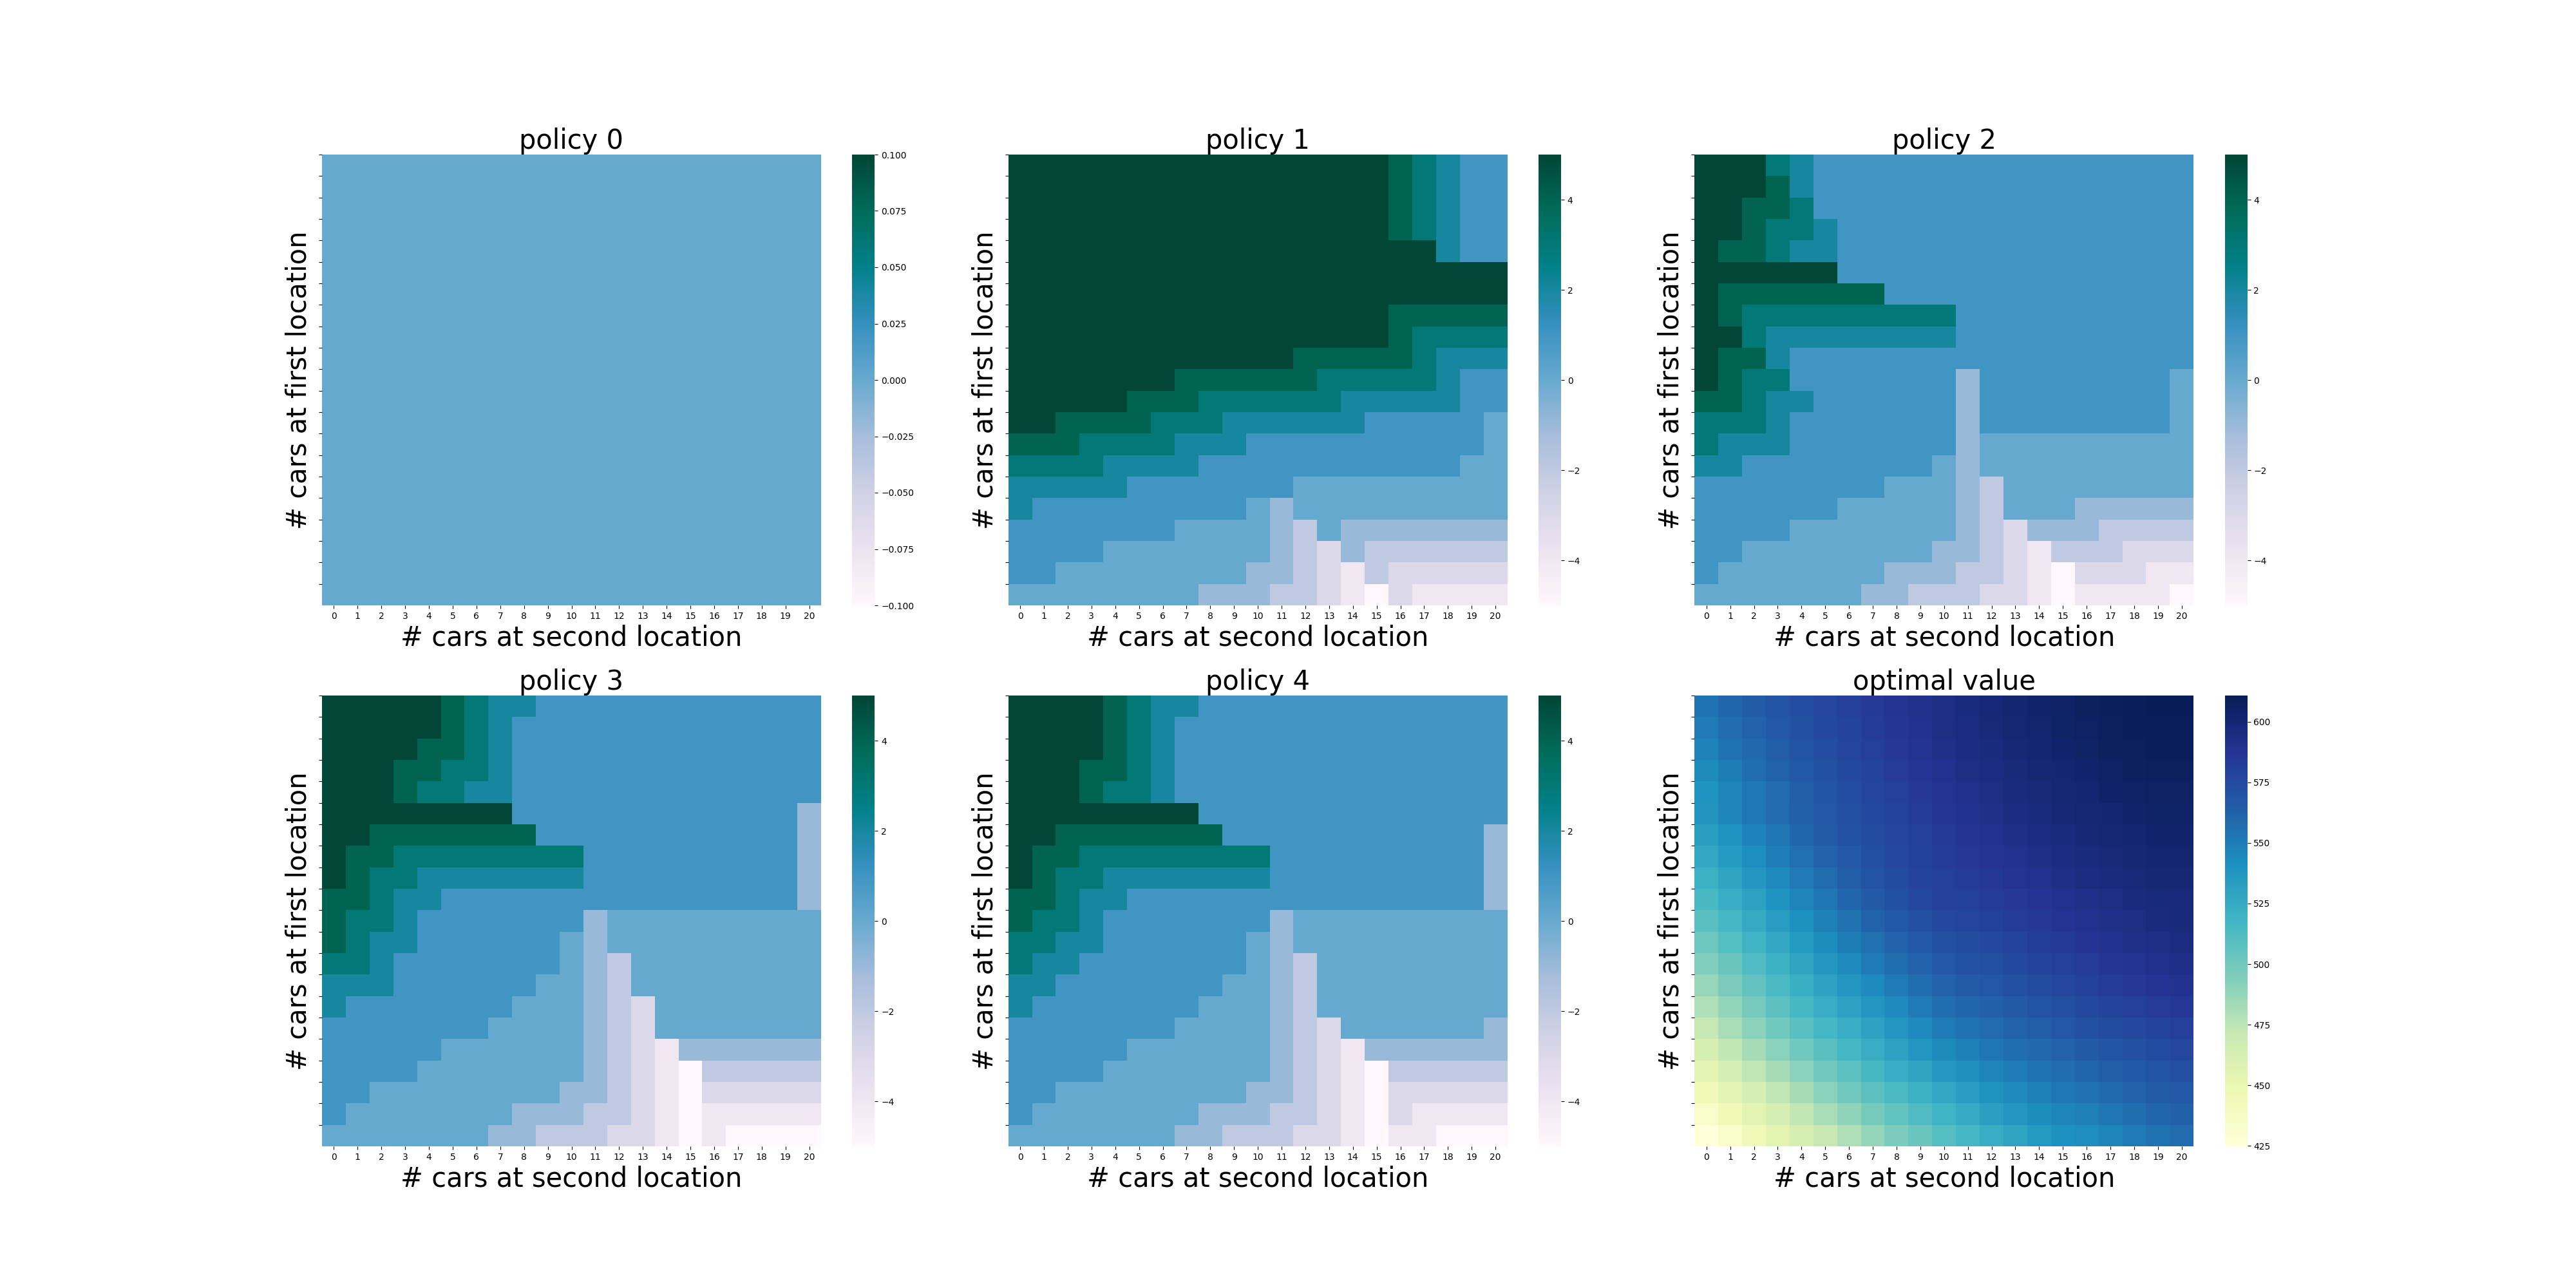
\includegraphics[scale=0.15]{figure_4_2_e_4_7}

    Parking fee encourages moving the cars around.
    This is more obvious for moving to 2nd location due to the first free car moved.

    \subsection{Question}

    Why does the optimal policy for the gambler’s problem have such a curious form?
    In particular, for capital of 50 it bets it all on one flip, but for capital of 51 it does not.
    Why is this a good policy?

    \subsection*{Answer}

    The coin is not fair and odds are against the gambler.
    As the number of flips increases the probability of winning decreases.
    The gambler must play with the least number of flips possible.
    Thus the gambler should bet all of his money when it is possible to reach the target quickly.
    Otherwise, the gambler bet minimum amount of money not to lose his chance of winning.

    With capital 50 the gambler should bet all its capital to reach target in one flip.
    With capital 51, with the optimal policy presented in the book, the gambler may bet 1 so that if he loses he would still be able to try the target with remaining capital 50.

    The family of optimal solutions forms a triangle enclosing the presented solution.
    There are many optimal solutions because it is possible to reach the target with different amounts in the same number of flips.
    The presented solution forms the lower bound of the optimal policy families.
    This is probably due to using the first value returned by the argmax function.


    \subsection{Question}

    (programming) Implement value iteration for the gambler’s problem and solve it for ph = 0.25 and ph = 0.55.
    In programming, you may find it convenient to introduce two dummy states corresponding to termination with capital of 0 and 100, giving them values of 0 and 1 respectively.
    Show your results graphically, as in Figure 4.3.
    Are your results stable as theta goes to 0?

    \subsection*{Answer}

    {\red Solo revisé la respuesta en el PDF, no el programa.}

    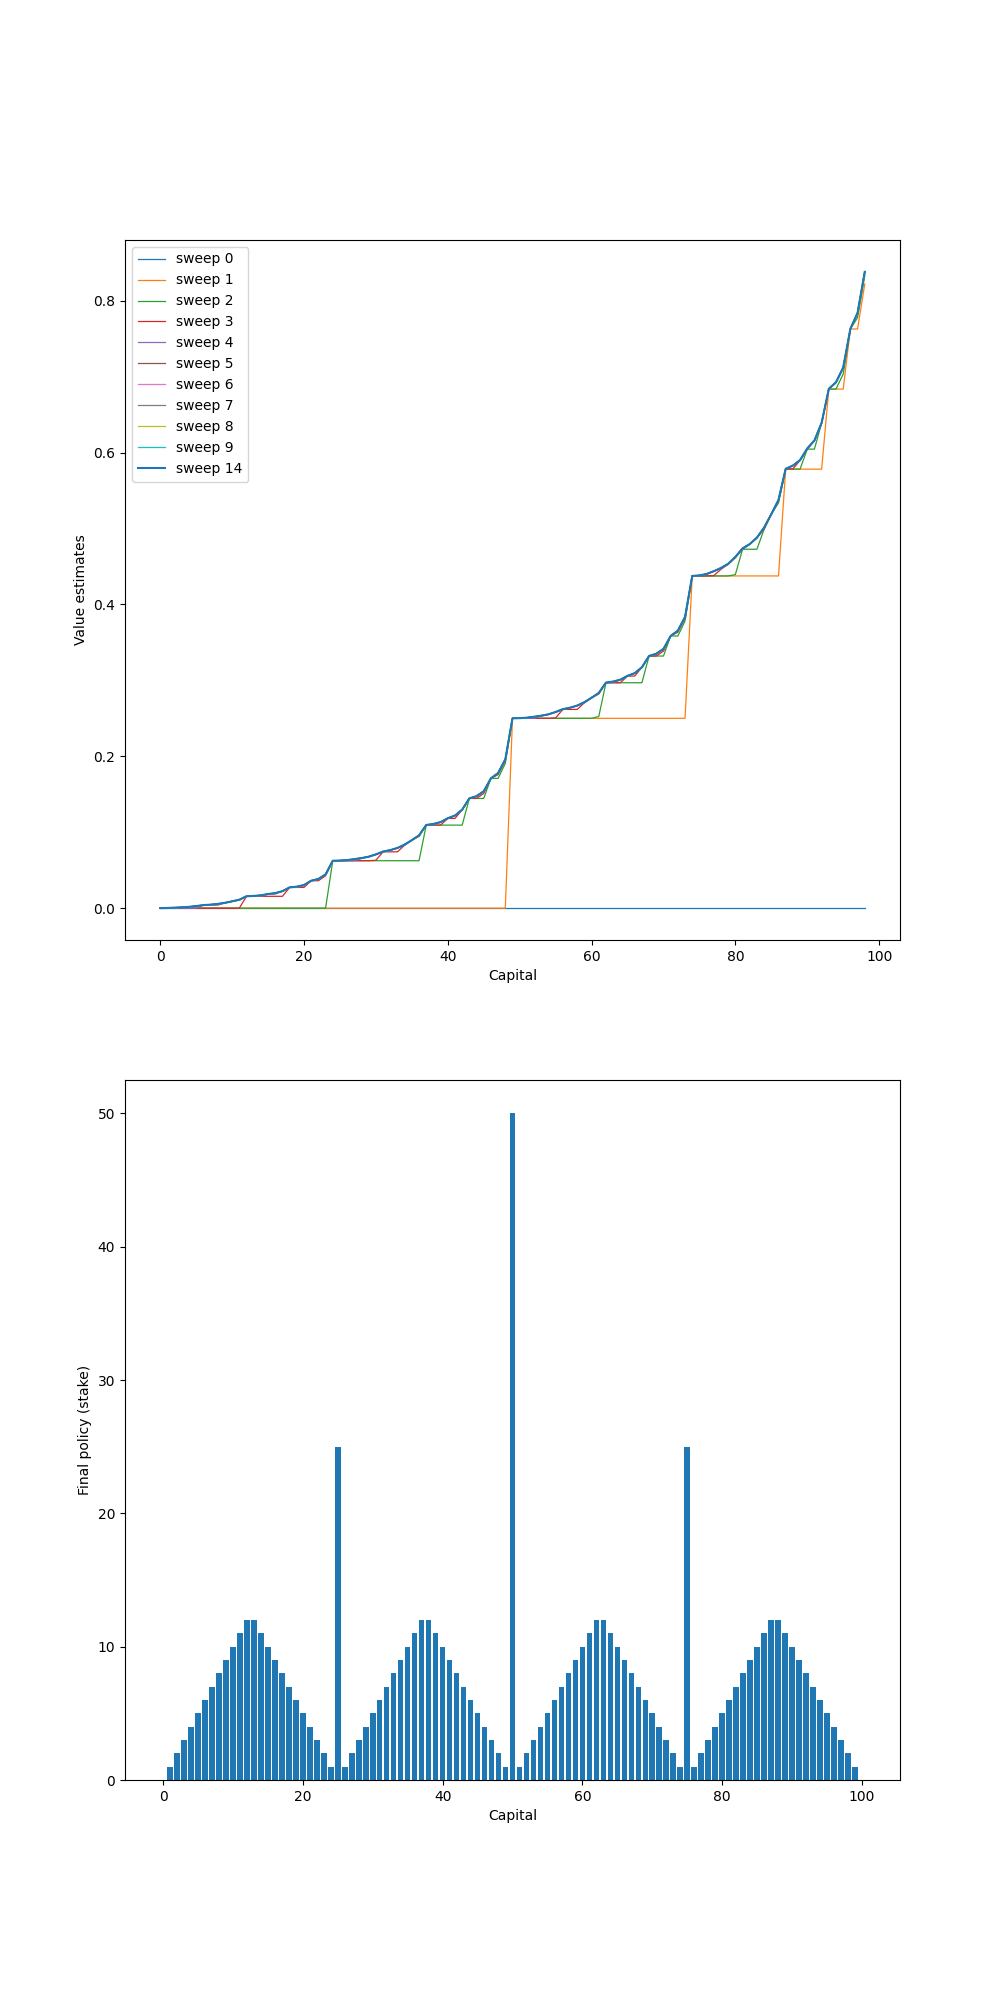
\includegraphics[scale=0.4]{figure_4_3_e_4_9_p25}

    Ph 0.25 gives similar results to Ph 0.4. This is expected because both cases disfavors the gambler.

    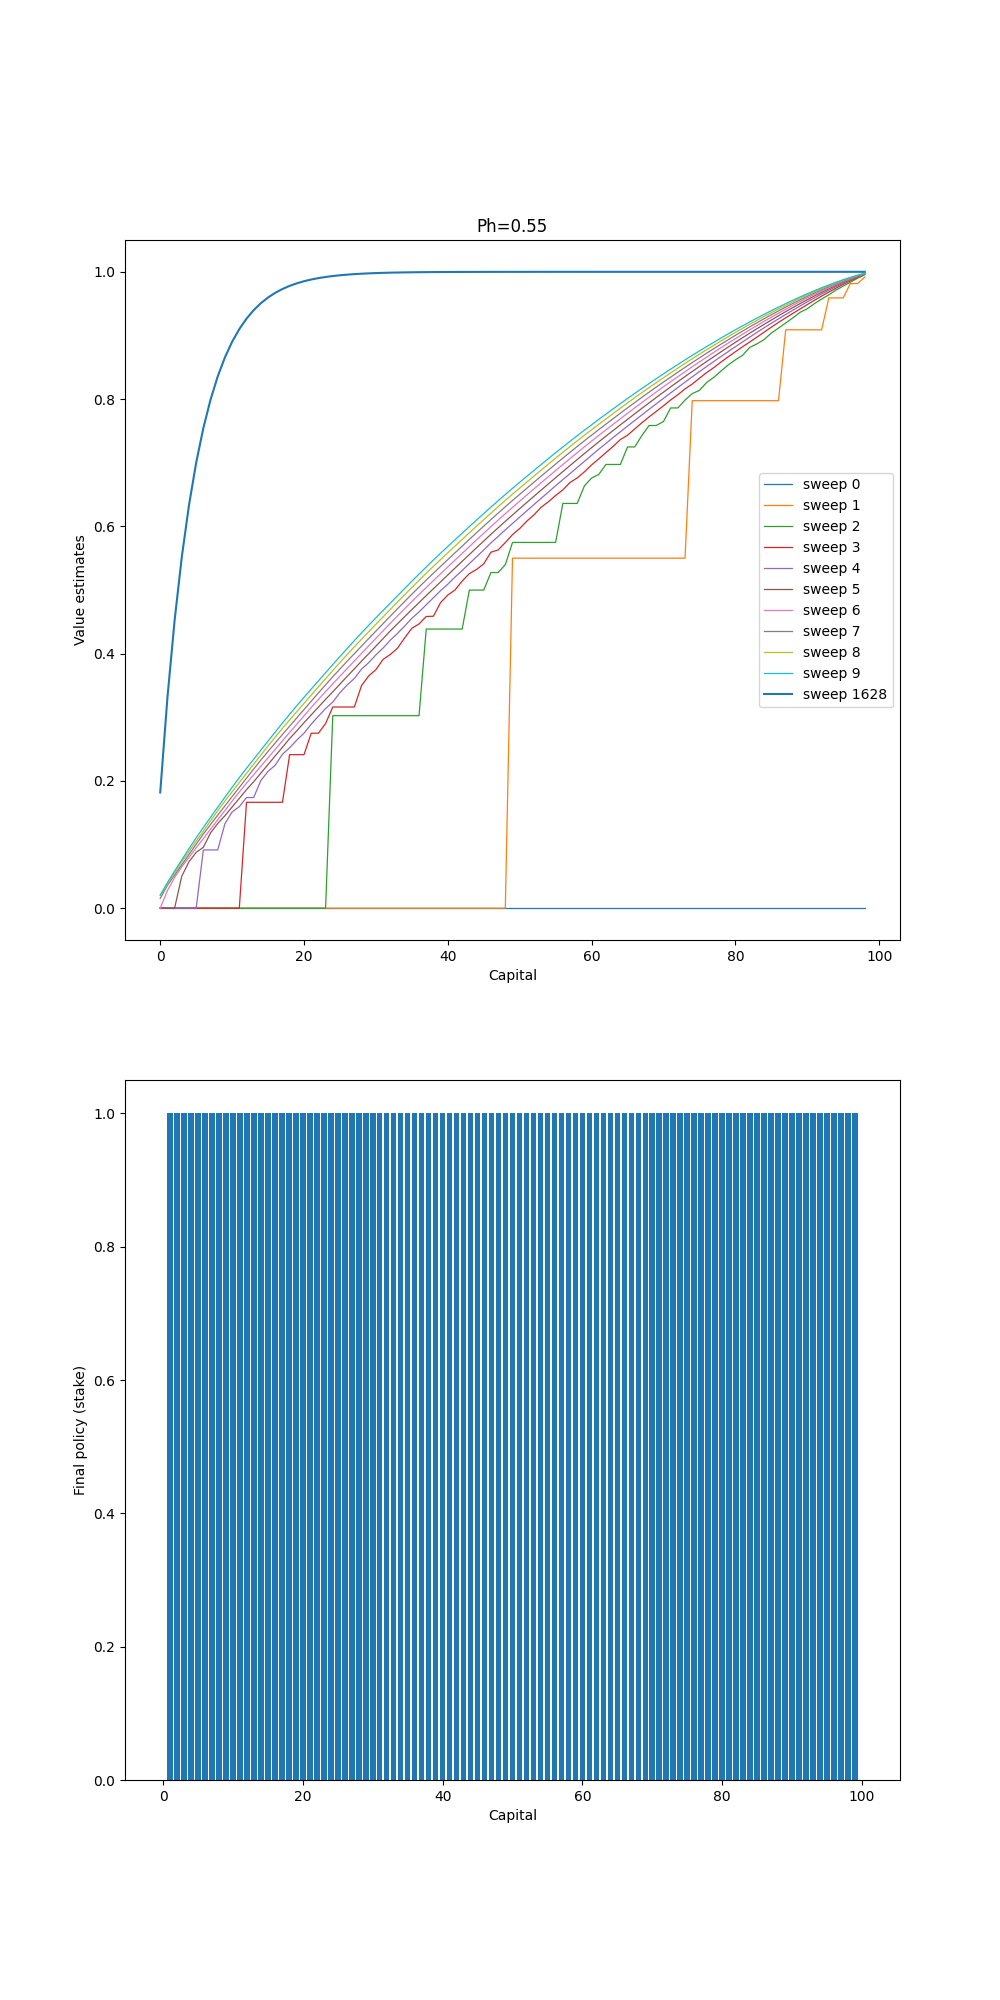
\includegraphics[scale=0.4]{figure_4_3_e_4_9_p55}

    Ph 0.55 encourages longer plays.
    The gambler uses small stake increments to limit losing.

    As theta approaches to zero, results remain stable but number of sweeps needed to stabilize is raised.

    \subsection{Question}

    What is the analog of the value iteration update (4.10) for action values, q k+1 (s, a)?

    \subsection*{Answer}

    See equation \ref{eqn:eq4_5} for reference.

    \begin{equation}
        q_{k+1}(s, a) = \sum_{s',r} p(s', r | s, a) [r + \gamma \max_{a'} q_k(s', a')]
    \end{equation}

\end{document}